\section{Preparation}
\subsection{What is coherent light?}
\begin{itemize}
    \item well defined ohase relationship
    \item one single wavelength
\end{itemize}

\subsection{How do you get population inversion?}
\begin{itemize}
    \item electrical pumping of the semiconductor
\end{itemize}

\subsection{How does light amplification in p-n diodes work?}
\begin{itemize}
    \item electron and hole recombinate 
    \item stimulated photon emission
\end{itemize}

\subsection{What are the differences in electronics structure 
between metals, semiconductors and isolators. Explain it with 
the help of valence and conduction bands.}
\begin{itemize}
    Metals:
    \item Valence Band: partially filled with electrons
    \item Conduction band: Overlapping with the valence band, containing free electrons
    Semiconductors:
    \item Valence Band: Fully filled with electrons
    \item Conduction Band: Seperated form the valence band by a small energy gap
    \item Electrons can jump from the valence in the conduction band
    \item Limited free electrons in the conduction band at room temperature
    Isolators:
    \item a Semiconductor with a large energy gap
    \item no electrons in the conduction band 
\end{itemize}

\subsection{What is a p- and n-doped semiconductor?}
\begin{itemize}
    p-doped:
    \item add atoms with less valenceelectrons
    \item creates extra holes
    n-doped:
    \item add atoms with more valenceelectrons
    \item creates extra electrons
\end{itemize}

\subsection{Discuss the working principle of a diode laser.}
\begin{itemize}
    \item Semiconductor with p-n junction
    \item Electric field causes population inversion
    \item Electrons recombine with holes in the p-type region and emit a photon
    \item Photons stimulate this process for other electrons-hole pairs
    \item Photons from stimulated emission are coherent
    \item Mirrors on both sites provide more and more coherent photons, resulting in a laserbeam
\end{itemize}
\subsection{Disscuss the internal and external cavity of a diode laser.}
\begin{itemize}
    internal cavity
    \item necessary for the laser (stimulated emission)
    external cavity
    \item serves to  frequency-stabilize and line narrows the laser output
\end{itemize}
\subsection{What is the Littrow configuration?}
\begin{itemize}
    \item diffracted light is retroreflected back alsong the same path as the 
    incident light using a diffraction grating
    \item used to select a specific wavelength
    \item useful for tunung and stabilizing the laser
\end{itemize}
\subsection{Which laser modes can be get?}
\begin{itemize}
    \item ???
\end{itemize}
\subsection{Explain the concept of 'mode hopping'.}
\begin{itemize}
    \item ???
\end{itemize}
\subsection{What defines the wavelength of a diode laser?}
\begin{itemize}
    \item the energygap of the semiconductor
    \item temperature
    \item injection current
\end{itemize}
\subsection{To which class of materials does rubidium belong?}
\begin{itemize}
    \item alkali metals
\end{itemize}
\subsection{What splitting are caused by an external magnetic field?}
\begin{itemize}
    \item Hyperfine structure (quantum number $F$)
\end{itemize}
\begin{figure}
    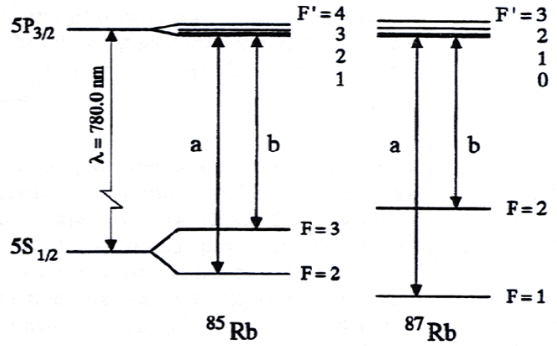
\includegraphics{pictures/Zeeman.png}
\end{figure}
\subsection{Calculate the hyperfine splitting of rubidium}
\begin{itemize}
    \item ???
\end{itemize}
\subsection{What are the selection rules for magnetic dipole transitions?}
\begin{itemize}
    \item $\Delta J = -1,0,+1$
    \item $\Delta M = -1,1$
\end{itemize}
\subsection{What does absorption sectroscopy mean?}
\begin{itemize}
    \item measure the amount of light absorbed by a material as a function of the wavelength
    \item provides information about the electronic and molecular structure of the material
\end{itemize}